\subsection*{Database}
Databasen kan tilgås ved den tilhørende controller. Databasen og controlleren fremgår af \autoref{fig:MVCDatabase}. 

\begin{figure} [H]
\centering
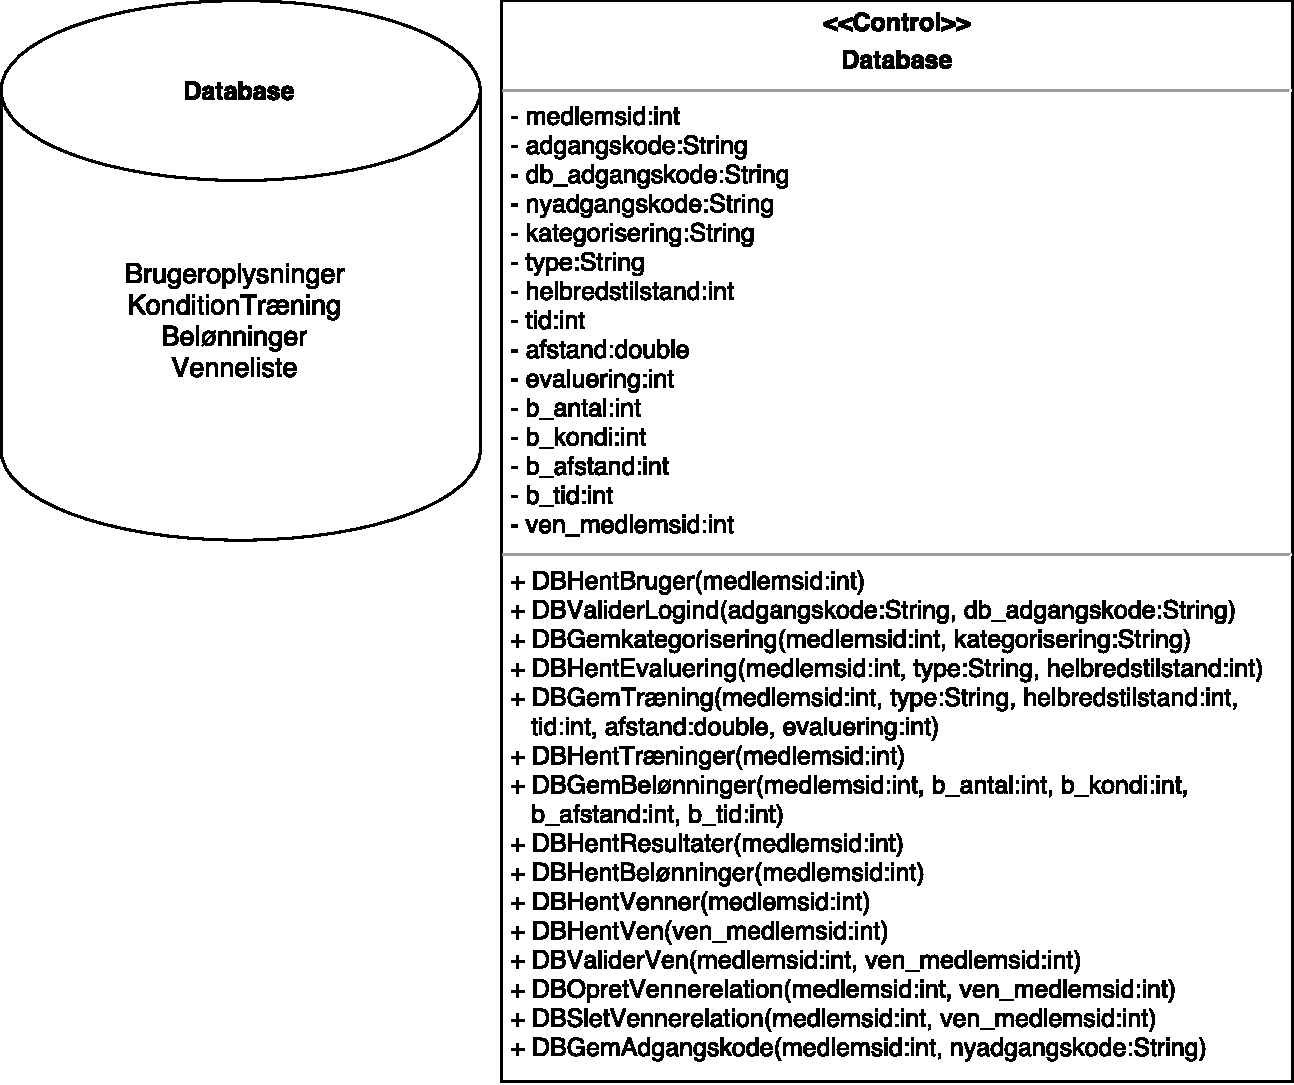
\includegraphics[width=0.5\textwidth]{figures/MVC/MVCDatabase}
\caption{Designklasser for Database.}
\label{fig:MVCDatabase}
\end{figure}

\noindent
Databasen indeholder brugeroplysninger, venneliste, resultater og registrerede brugere. Designet af denne vil fremgå af \autoref{sec:ER}. \textit{DatabaseController} har til formål at gemme, sende og modtage data mellem databasen og de forskellige controllere. Der oprettes forbindelse til denne ved log ind, hvor brugeroplysninger, venneliste og resultater sendes og gemmes i de forskellige entity. 


\subsection*{Entity}  
Databasen har oprettet forbindelse ved log ind, sendes og gemmes data i tre forskellige entity, som fremgår af \autoref{fig:MVCEntity}. 

\begin{figure} [H]
\centering
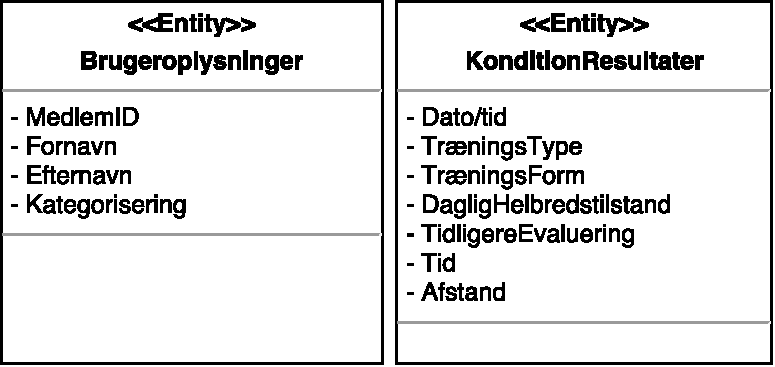
\includegraphics[width=0.9\textwidth]{figures/MVC/Entity}
\caption{Designklasser for Entity.}
\label{fig:MVCEntity}
\end{figure}

\noindent
\textit{Brugeroplysninger} indeholder informationer om brugeren, herunder MedlemsID, Adgangskode, Fornavn, Efternavn og Kategorisering. Denne har en relation med RedigeringController, som fremgår af \autoref{fig:MVCRedigering}. 
\textit{Venneliste} har informationer om andre brugere der følges, såsom VenMedlemsID, VenFornavn, VenEfternavn og VenBelønninger. Controllerne der har relationen til denne beskrives i \autoref{fig:MVCVenneliste} og  \autoref{fig:MVCVen}.
\textit{Resultater} indeholder brugerens resultater, som er defineret ud fra DatoTid, TræningsType, TræningsForm, DagligHelbredstilstand, Evaluering, Tid, Afstand, KompatibleMålinger og Belønninger. Disse har relation til ResultatController, der fremgår af  \autoref{MVCResultat}.

